\section{Patron de reconfiguration}

\begin{frame}{Critères de réutilisation des décisions de reconfiguration}
\begin{itemize}
\setlength\itemsep{0.7cm}
\item \textbf{Titre} : méthaphore                                                                   
\item \textbf{Intention} : description générale                                                                   
\item \textbf{Contexte} : hypothèse de la solution                                                                    
\item \textbf{Problème} : besoins à satisfaire                                                                     
\item \textbf{Solution} : résolution du problème                                                                     
\item \textbf{Conséquence} : description effets sur les aspects non
fonctionnels                                                              
\end{itemize} 
\end{frame}


\begin{frame}[fragile]{Type de documentation des décisions : docu.
formelle \emph{Allen, 1998}}
\centering
\begin{figure}
\begin{subfigure}[b]{0.4\textwidth}
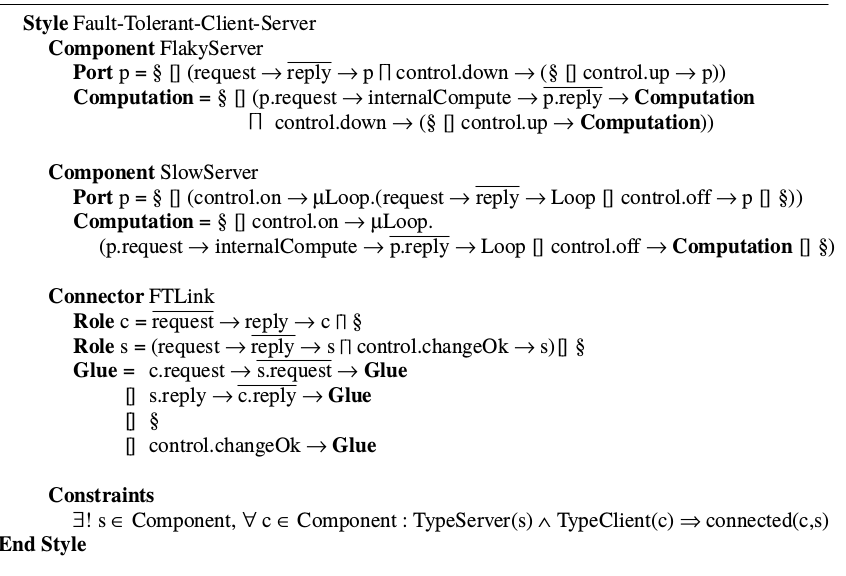
\includegraphics[width=5cm]{imgs/slide_fault-tolerance.png}
\caption{Contexte et problème}
\end{subfigure}
\begin{subfigure}[b]{0.4\textwidth}
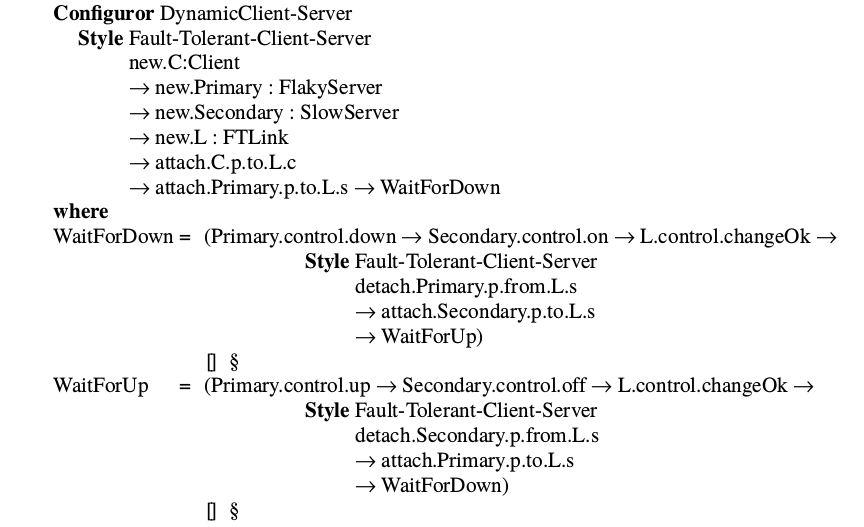
\includegraphics[width=5cm]{imgs/slide_reconf_specif.png}
\caption{Solution}
\end{subfigure}
\end{figure}

\begin{table}[]
\resizebox{0.85\textwidth}{!}{%
\begin{tabular}{ccccccc}
         & Titre     & Intention & Contexte  & Problème  & Solution  & Conséquence \\
Allen    & \textcolor{red}{\ding{53}} & \textcolor{red}{\ding{53}} &
\ding{51} & \ding{51} & \ding{51} & \textcolor{red}{\ding{53}}   \\ 
\end{tabular}}
\end{table}
\end{frame}

\begin{frame}[fragile]{Type de documentation des décisions : docu. formelle
\emph{Oliveira, 2015}}
\centering
\begin{figure}

\includegraphics[width=8cm]{imgs/slide_oliveira_primitive.png}
\caption{Contexte}
\end{figure}
\begin{figure}
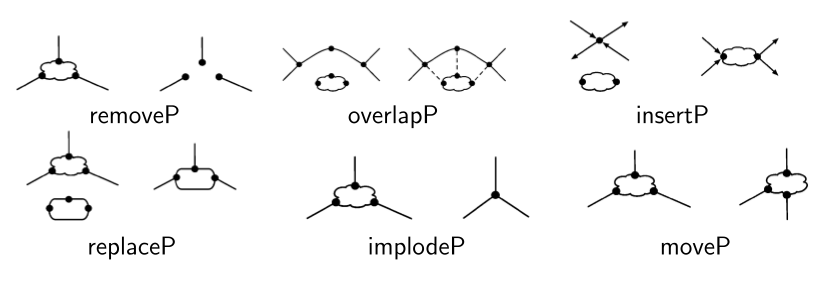
\includegraphics[width=8cm]{imgs/slide_oliveira_patron.png}
\caption{Problème}
\end{figure}
\begin{table}[]
\resizebox{0.85\textwidth}{!}{%
\begin{tabular}{ccccccc}
         & Titre     & Intention & Contexte  & Problème  & Solution  & Conséquence \\
Oliveira & Partielle & \ding{53} & \ding{51} & Partielle & Partielle & \ding{53} \\
\end{tabular}}
\end{table}
\end{frame}

\begin{frame}[fragile]{Type de documentation des décisions : docu.
semi-formelle
\emph{Gomaa, 2004}}
\textbf{Titre :} Master-Slave Reconfiguration Pattern, Centralized Control
Reconfiguration Pattern, Client / Server Reconfiguration Pattern,
Decentralized Control Reconfiguration
Pattern.
\begin{figure}
\begin{subfigure}[b]{0.5\textwidth} % "0.45" donne ici la largeur
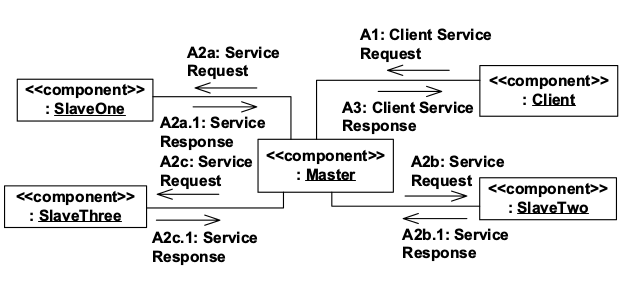
\includegraphics[width=3cm]{imgs/gomaa_contexte}
\caption{Contexte}\label{fig:orchid}
\end{subfigure}
\begin{subfigure}[b]{0.5\textwidth} % "0.45" donne ici la largeur
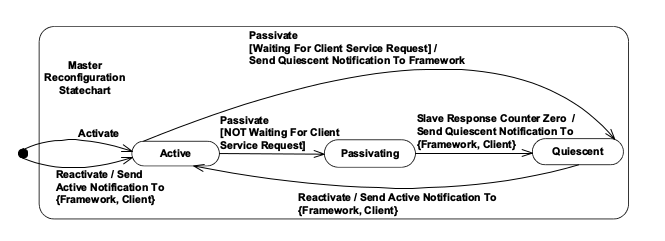
\includegraphics[width=3cm]{imgs/gomaa_solution}\\
\caption{Solution}\label{fig:orchid}
\end{subfigure}
\end{figure}
\begin{table}
\resizebox{0.85\textwidth}{!}{%
\begin{tabular*}{\textwidth}{c @{\extracolsep{\fill}} ccccccc}
         & Titre     & Intention & Contexte  & Problème  & Solution  & Conséquence \\
Gomaa    & Partielle & Partielle & \ding{51} & \ding{53} &\ding{51}  & \ding{53}   \\
\end{tabular*}}
\end{table}
\end{frame}
%
\begin{frame}{Comparaison des caractéristiques des décisions de reconfiguration
pour les SdSs}
\begin{table}[]
\centering
\resizebox{0.85\textwidth}{!}{%
\begin{tabular*}{\textwidth}{c @{\extracolsep{\fill}} ccccccc}
         & Titre     & Intention & Contexte  & Problème  & Solution  & Conséquence \\
Allen    & \ding{53} & \ding{53} & \ding{51} & \ding{51} & \ding{51} & \ding{53}   \\
Oliveira & Partielle & \ding{53} & \ding{51} & Partielle & Partielle & \ding{53}   \\
Gomaa    & Partielle & Partielle & \ding{51} & \ding{53} &\ding{51}  & \ding{53}   \\
\end{tabular*}
}
\end{table}
\end{frame}


\begin{frame}{Patron de reconfiguration co-évolution : délimitation du problème}
\begin{figure}
\begin{subfigure}[b]{0.4\textwidth}
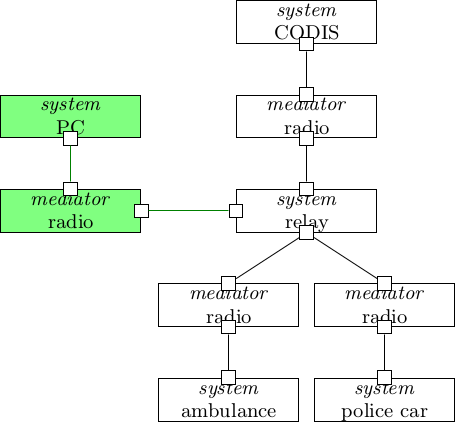
\includegraphics[height=2.5cm]{imgs/fig_rearchitecture}
\caption{Contexte}
\end{subfigure}
\begin{subfigure}[b]{0.4\textwidth}
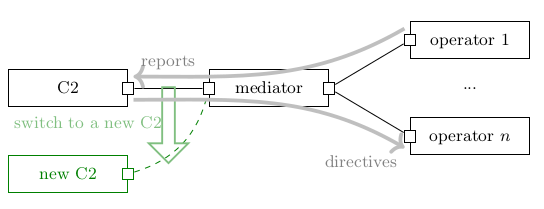
\includegraphics[width=4cm]{imgs/dc_archi-C2}
\caption{Problématique}
\end{subfigure}
\end{figure}

Invariants :
\begin{itemize}
\item Les deux C2 partagent le même état de mission.
\item Tous les opérateurs sont connectés à exactement un
C2. 
\end{itemize}

Forces :
\begin{itemize}
\item Instancier une deuxième version du composant qui coexiste avec
la version initiale.
\item Synchroniser les états partagés entre les versions du
composant.
\end{itemize}

\end{frame}

\begin{frame}{Patron de reconfiguration : description de la solution}
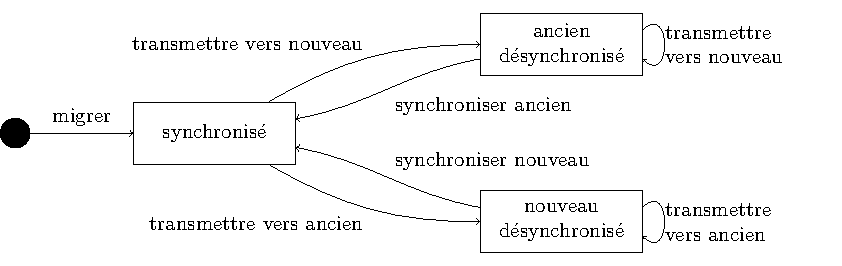
\includegraphics[width=12cm]{imgs/slide_solution_coevolution.pdf}
\end{frame}

\begin{frame}{Amélioration de la réutilisation}
\end{frame}

\begin{frame}{Résumé}
\begin{itemize}
\setlength\itemsep{0.7cm}
\item \underline{\textbf{Quiescence}} : rendre passif,
les composants dépendant du composant ciblé par la reconfiguration. 
\item \underline{\textbf{Tranquilité}} : variante de la quiescence qui assouplie
les critères de reconfiguration. Elle décrit les conditions dans
lesquelles la reconfiguration peut-être réalisée sans attendre l'état de
quiescence
\item \underline{\textbf{Co-evolution}} : déployer directement la nouvelle version du composant ciblé par la
reconfiguration. Les deux versions d'un
composant s'executent simultanément. 
\item \underline{\textbf{Opportuniste}} : une opération de
déconnexion et connexion qui est réalisée dès que l'occasion se
présente.  
\end{itemize}
\end{frame}
